
\documentclass{article}
\usepackage{ijcai11}
\usepackage[dutch]{babel}
\usepackage{times}
\usepackage{gensymb}
\usepackage{graphicx}
\usepackage{float}
\usepackage{cite}
\usepackage{named}
\usepackage{url}


\title{Smart LED-displays}
\author{Barbara Ameloot\\
KU Leuven\\
barbara.ameloot@student.kuleuven.be
\And 
Wouter Jochems\\
KU Leuven\\
wouter.jochems@student.kuleuven.be}


\begin{document}

\maketitle

\begin{abstract}
Deze paper onderzoekt een mogelijke toepassing van smart LEDs, LEDs aangestuurd door een micro\-controller. Specifiek bestuderen we hun mogelijkheden op het gebied van LED-displays. LED-displays komen veel voor en in alle soorten en maten. Helaas zijn ze vooral zeer statisch. Ook hebben problemen met de verbinding tussen LEDs en het besturingselement al snel catastrofale gevolgen voor de bruikbaarheid van het display. Het gebruik van smart LEDs zou hier verandering in kunnen brengen. We concluderen dat smart LED-displays niet altijd een goede vervanging zijn voor conventionele LED-displays, maar wel extra mogelijkheden bieden voor meer experimentelere LED-displays.
\end{abstract}

{\bf Keywords:} smart LED, VLC, LED Display


\section{Introductie}

LED-displays worden tegenwoordig vaak gebruikt op evenementen en reclameborden. Deze werken steeds met een centrale verwerkingseenheid. Als er problemen opduiken met deze eenheid of met de verbinding tussen de LEDs en de controller, dan wordt meteen een groot deel van het scherm buiten werking gesteld\cite{brokenDisplay}. Ook beperkt de nood aan verbinding tussen controller en LEDs de mogelijkheden van het display. 
\begin{figure}[H]
\centering
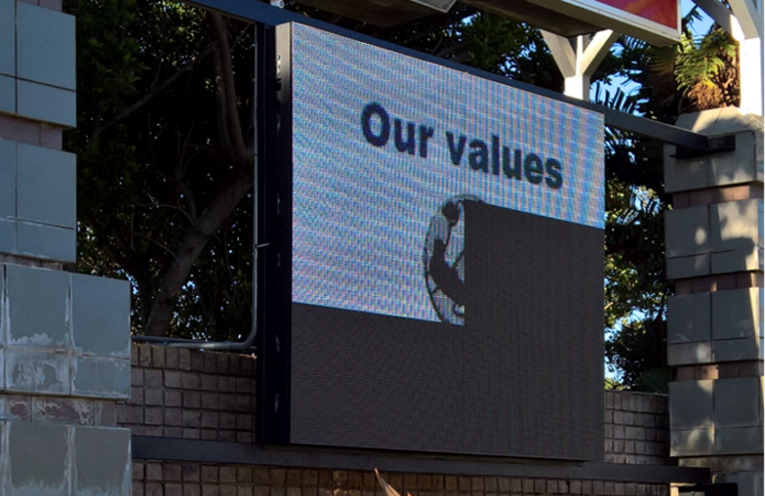
\includegraphics[width=7cm]{broken.png}
\caption{Een LED-display met verbindingsproblemen}
\end{figure}
Smart LEDs kunnen een oplossing bieden voor deze problemen. Elke LED beschikt namelijk over zijn eigen microcontroller. Dit voorkomt dat bij een fout een groot deel van het display onbruikbaar wordt. Ook kunnen de verschillende LEDs ten opzichte van elkaar bewegen zonder dat er kabels in de knoop raken of radiogolven met elkaar interfereren. Daarnaast kunnen smart LEDs samen werken door met elkaar te communiceren. Dit gebeurt via VLC (\textit{Visual Ligth Communication}). Hiervoor gebruiken ze hun ingebouwde LED die zowel als zender als als ontvanger kan dienen. 


\section{Verwant werk}
Dit project is een vervolg van het project van vorig jaar waarin de smart LEDs ontwikkeld werden. 


\section{Probleemstelling}

Het doel van ons onderzoek is het bekomen van een LED-display opgebouwd uit smart LEDs. We gaan na welke problemen opduiken en bedenken hier oplossingen voor. Uiteindelijk stellen we ons de vraag: bieden led displays opgebouwd uit smart LEDs een meerwaarde ten opzichte van conventionele LED displays? 

\smallskip

Hoe definiëren wij een meerwaarde:
\begin{itemize}
\item Smart LED-displays kunnen dienen als vervanging voor conventionele LED-displays
\begin{itemize}
\item Het Display werkt als 1 geheel
\item Het Display werkt onder alle licht omstandigheden
\end{itemize}
\item Smart LED-displays hebben minstens 1 extra voordeel ten op zichte van conventionele LED-displays
\end{itemize}

\smallskip


\section{Implementatie}
Om onze hypothese te testen maakten we gebruik van LEDs verbonden met Zigduino r2 microcontrollers. We maakten gebruik van infrarood LEDs voor de communicatie om extra licht flikkeringen in het display te voorkomen en om interferentie van de omgeving zo veel mogelijk te vermijden.


\section{Oplossing}

\subsection{Onderlinge communicatie}
Om een vlak display te bekomen, moeten de LEDs uiteraard zijdelings staan. Dit zorgde helaas voor problemen, aangezien elke LED een specifieke invalshoek heeft. Wij hadden echter geen LEDs met een hoek van 180\degree ter beschikking. Als oplossing probeerden we een diffuser te gebruiken maar hierdoor verzwakte het licht van onze LEDs waardoor er geen signaal kon worden verzonden. Mogelijk zou dit geen probleem zijn bij sterkere LEDs maar deze zouden problemen kunnen geven omdat ze teveel energie vragen. 

Met twee naar elkaar gerichte LEDs lukt het ons wel om een bit-string door te zenden. Deze opstelling bestaat uit een eerste LED die een bit-string uitzend, een tweede die deze ontvangt en doorgeeft aan een microcontroller en vervolgens een derde die de ontvangen bit-string weer uitzend in een andere richting. In minder conventionele LED-displays (met een vorm die het toelaat de LEDs naar een elkaar te richten of met bewegende onderdelen) is onderlinge communicatie dus wel mogelijk.

\subsection{Meerdere LEDs}
Bij aanvang van ons project hoopten we voor het display en het verzenden van informatie dezelfde LED te gebruiken. Dit is niet alleen compacter dan met meerdere LEDs maar het zorgt er ook voor dat we de smart LED niet moeten uitbreiden met extra hardware. Helaas bracht dit extra moeilijkheden met zich mee, zoals informatie die verzonden moest worden over een LED die volgens het display geen licht mag uitzenden. Ook maakte dit onze code veel complexer. Hierdoor kozen we om met een tweede LED te werken. Om er voor te zorgen dat de communicatie-LEDs geen signalen zouden opvangen van de display-LEDs besloten we om de communicatie via een infrarood LED te laten verlopen. Dit hielp ook meteen met het omgevingslicht probleem. 

\subsection{Externe lichtbron}
Omdat een tweede LED ook een externe lichtbron is, valt uit het voorgaande al te besluiten dat een goed gericht licht in staat is om te interageren met een smart LED-display. Wij maakten gebruik van een afstandsbediening die naargelang welke knop werd ingeduwd, een ander stukje code uitzond.

\subsection{Omgevingslicht}
Om ervoor te zorgen dat het programma meer omgevingslicht niet als een signaal zou herkennen, voegden we een dynamische threshold toe.
Onze huidige aanpak neemt bij elke iteratie het gemiddelde van een tiental metingen. Deze waarde wordt vergeleken met de vorige threshold, zo wordt vermeden dat een te hoge waarde wordt aangenomen als er tijdens de metingen al een signaal verzonden wordt.
We merkten op dat bij deze aanpak de threshold zeer veel veranderde. Bij het visualiseren van deze ruis was een duidelijk sinusoïdaal verloop te zien. Dit is te verklaren aan de hand van de spoelen en condensatoren in de microcontroller die constant opladen en ontladen. Eventueel kan hier rekening mee gehouden worden om een nog accuratere threshold te bekomen.


\section{Conclusie}
We concluderen dat smart LED-displays geen alternatief zijn voor conventionele LED-displays maar dat ze toch over bepaalde eigenschappen beschikken die ze niet alleen bruikbaar maar ook bijzonder maken. Ze kunnen interactief gebruikt worden als simpele, vlakke displays zonder onderlinge communicatie maar ook zonder eventuele verbindingsproblemen. Daarnaast kunnen ze in andere vormen wel signalen doorgeven en dus meer als 1 geheel functioneren.


\section{Verder werk}
Als vervolg op dit project zou een display opgebouwd uit echte smart LEDs gemaakt kunnen worden. Het zou ook interessant zijn mocht er een oplossing gevonden worden voor het probleem met de invalshoek van de LEDs zodat zijdelings gecommuniceerd kan worden. Verder is er nog de reeds voorgestelde aanpassing aan de threshold die rekening zou kunnen houden met de sinusoïdale ruis.


\bibliographystyle{named}
\bibliography{bronnen}

\end{document}

